\title[Swiss STACK User Meeting 2025]{Swiss STACK User Meeting 2025}

\subtitle{standardized testing and\\
	a sneak peek into our workflow with STACK} % Correction here: "a sneak peek"

\author
{
	\mainauthorA, \and	Michael Anderegg, \and \mainauthorB
}

\institute[KLW]
{
	Department of Informatics\\
	Kantonsschule (high school) Im Lee, Winterthur
}

\date{10. June 2025}

\logo{
\includegraphics[width=3cm]{Logos/LeeLogo}}

\frame{\titlepage}

\begin{frame}{Thank you!}
	\begin{itemize}
		\item It is a pleasure to work with good tools.
		      \pause
		\item STACK, Moodle and Maxima very much belong to that category of tools.
	\end{itemize}
\end{frame}

\begin{frame}{contents of this short talk}
	\begin{itemize}
		\item standardized testing in mathematics at our school % Suggestion: clearer wording
		      \pause
		\item our workflow to create STACK-questions
	\end{itemize}
\end{frame}

\begin{frame}{standardized testing}
	\begin{itemize}
		\item We have created a fair number ($100+$) of STACK-questions, covering most topics in mathematics of the first 2 years at our school.
		      \pause
		\item The questions contain radomization.
		      \pause
		\item The students get the chance to prepare for the exam using these questions!
		      \pause
		\item They can have Moodle generate mock exams based on these questions.
		      \pause
		\item The real exam is randomly generated individually for each student, following the same rules of generation as for the mock exams.
	\end{itemize}
\end{frame}

\begin{frame}{a few impressions}
	\begin{figure}[h!]
		\centering
		\hspace*{-1cm}
		\hfill % Adds horizontal space between minipages
		\begin{minipage}[c]{0.55\textwidth}
			\centering
			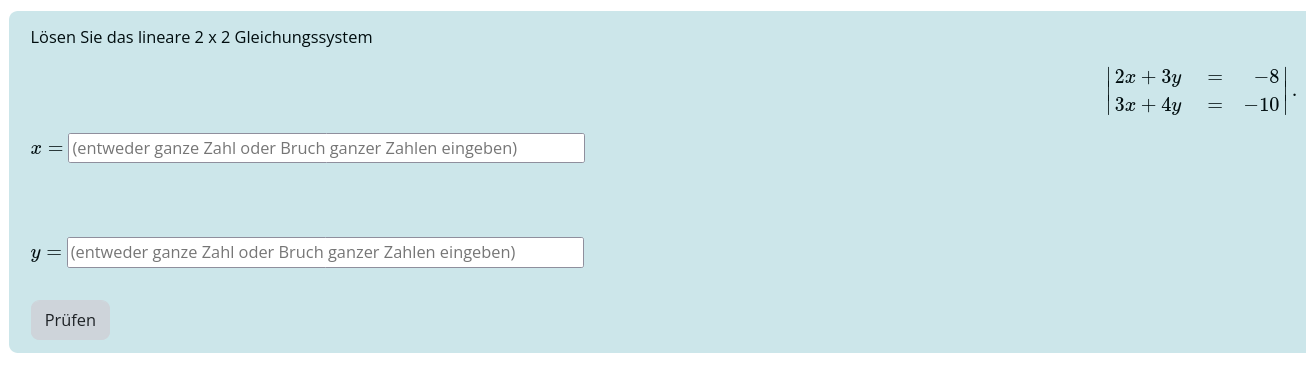
\includegraphics[width=\textwidth]{Various/ETH_STACK_Meeting_2025/Screenshots/example_question_0.png}
			% \caption{Caption for Image 2} % Optional caption
		\end{minipage}%
		\begin{minipage}[c]{0.55\textwidth}
			\centering
			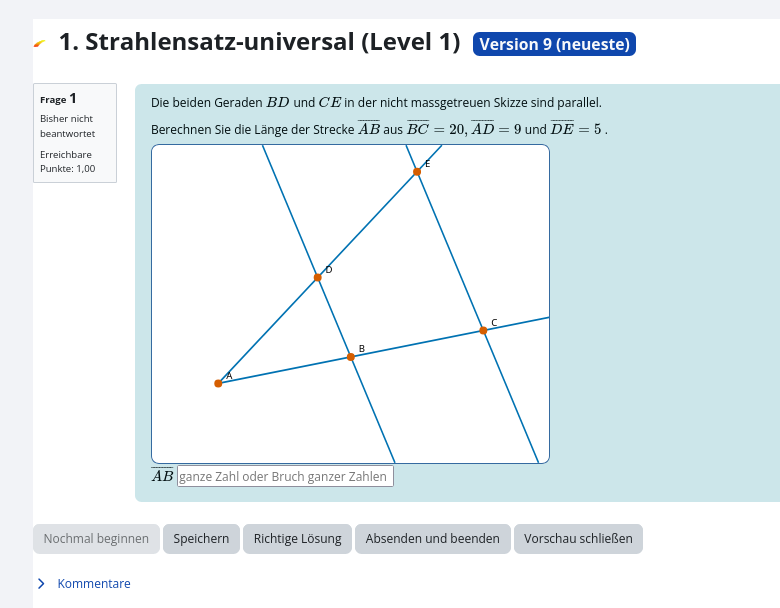
\includegraphics[width=\textwidth]{Various/ETH_STACK_Meeting_2025/Screenshots/example_question_1.png}
			% \caption{Caption for Image 2} % Optional caption
		\end{minipage}%
		\hfill
		\begin{minipage}[c]{0.55\textwidth}
			\centering
			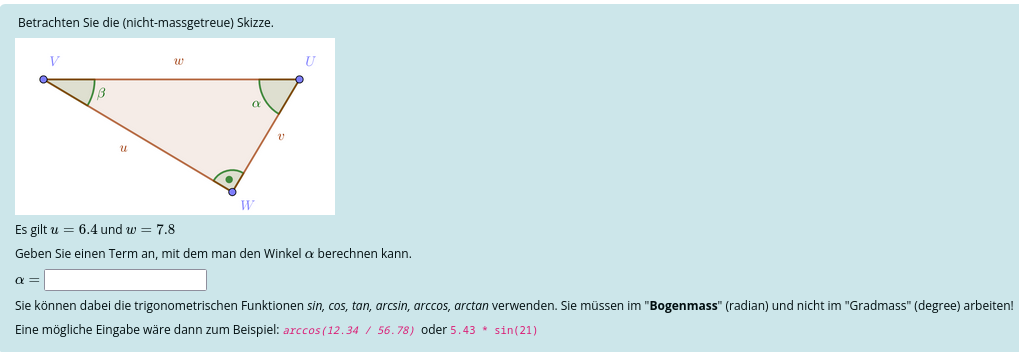
\includegraphics[width=\textwidth]{Various/ETH_STACK_Meeting_2025/Screenshots/example_question_2.png}
			% \caption{Caption for Image 3} % Optional caption
		\end{minipage}
	\end{figure}
\end{frame}

\begin{frame}{standardized testing}
	\begin{itemize}
		\item The exam take place for all students of the same year at the same time.
		      \pause
		\item We have already conducted this exam three times: 2023, 2024, 2025.
	\end{itemize}
\end{frame}



\begin{frame}{our workflow to create STACK-questions}
	\begin{itemize}
		\item We started by studying the documentation on Maxima and STACK.
		      \pause
		\item We were struggling to find comprehensive and involved examples at first.
		      \pause
		\item Chatbots / LLMs such as Gemini and ChatGPT have speed up the creation of STACK-questions significantly.
		      \pause
		\item It is useful to create custom GPTs for the creation of STACK-questions.
	\end{itemize}
\end{frame}

\begin{frame}{Discussion}
	\begin{itemize}
		\item questions? remarks? comments? suggestions?
		      \pause
		\item We have a few questions to this illustrious audience as well. \emoji{grinning-face-with-big-eyes}
	\end{itemize}
\end{frame}












